\documentclass{beamer}
\usepackage{beamerthemesplit}
\usepackage{wrapfig}
\usetheme{SPbGU}
\usepackage{pdfpages}
\usepackage{amsmath}
\usepackage{mathtools}
\usepackage{cmap} 
\usepackage[T2A]{fontenc} 
\usepackage[utf8]{inputenc}
\usepackage[english,russian]{babel}
\usepackage{indentfirst}
\usepackage{amsmath}
\usepackage{tikz}
\usepackage{multirow}
\usepackage[noend]{algpseudocode}
\usepackage{algorithm}
\usepackage{algorithmicx}
\usepackage{ stmaryrd }
\usepackage{qtree}
\usetikzlibrary{shapes,arrows}
\usepackage{fancyvrb}
\newtheorem{rutheorem}{Теорема}
\newtheorem{ruproof}{Доказательство}
\newtheorem{rudefinition}{Определение}
\newtheorem{rulemma}{Лемма}
\beamertemplatenavigationsymbolsempty

\newcommand{\derive}[0]{\xRightarrow[]{*}}
\newcommand{\derives}[0]{\xRightarrow[]{}}
\newcommand{\derivek}[1]{\xRightarrow[]{#1}}
\newcommand{\deriveg}[1]{\xRightarrow[#1]{*}}
\newcommand{\derivegone}[1]{\xRightarrow[#1]{}}

\title[]{Теория автоматов и формальных языков}
\subtitle[]{Контекстно-свободные языки}
\institute[]{
Санкт-Петербургский государственный электротехнический университет <<ЛЭТИ>>\\
}

\author[]{Екатерина Вербицкая}

\date{3 ноября 2017г.}

\definecolor{orange}{RGB}{179,36,31}

\begin{document}
{
  \begin{frame}
    \titlepage
  \end{frame}
}


\begin{frame}[fragile]
  \transwipe[direction=90]
  \frametitle{В предыдущей серии}
  \begin{itemize}
    \item Контекстно-свободные грамматики (все правила имеют вид $A \rightarrow \alpha$) 
    \item КС языки и разрешимость проверки пустоты
    \item Нормальная форма Хомского
    \item Алгоритм CYK
  \end{itemize}
\end{frame}

\begin{frame}[fragile]
  \transwipe[direction=90]
  \frametitle{В предыдущей серии: НФХ}
  КС грамматика находится в \textbf{нормальной форме Хомского}, если все ее правила имеют вид: 
  \begin{itemize}
    \item $A \rightarrow B C$, где $A,B,C \in V_N$
    \item $A \rightarrow a$, где $A \in V_N, a \in V_T$
    \item $S \rightarrow \varepsilon$, если в языке есть пустое слово, где $S$ --- стартовый нетерминал
  \end{itemize}

  \begin{enumerate}
    \item Удалить стартовый нетерминал из правых частей правил 
    \item Избавиться от неодиночных терминалов в правых частях 
    \item Удалить длинные правила (длины больше 2)
    \item Удалить непродуктивные правила ($\varepsilon$-правила)
    \item Удалить цепные правила
   \end{enumerate}
\end{frame}


\begin{frame}[fragile]
  \transwipe[direction=90]
  \frametitle{В предыдущей серии: CYK}
  \begin{itemize}
      \item Алгоритм синтаксического анализа, работающий с грамматиками в НФХ
      \item Динамическое программирование
  \end{itemize}

  \begin{center}
    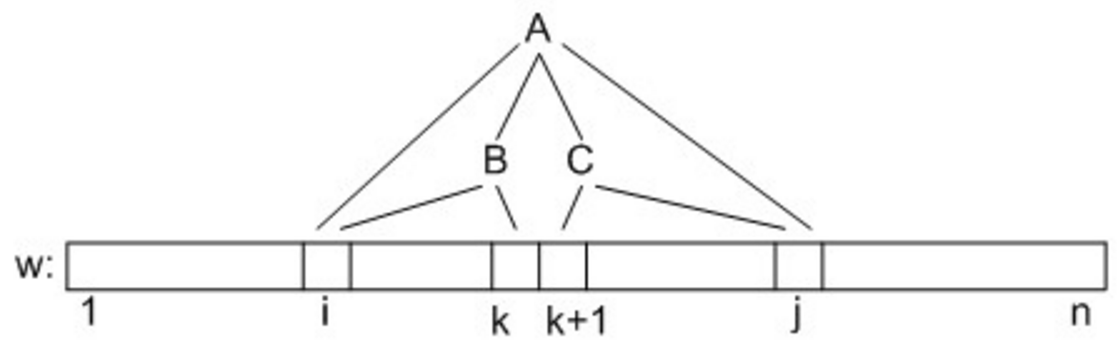
\includegraphics[width=\textwidth]{pics/CYK.png}  
  \end{center}
\end{frame}


\begin{frame}[fragile]
  \transwipe[direction=90]
  \frametitle{В предыдущей серии: CYK}
  \begin{itemize}
      \item Дано: строка $\omega$ длины $n$, грамматика $G = \langle V_T, V_N, P, S\rangle$ в НФХ
      \item Используем трехмерный массив d булевых значений размером $|V_N| \times n \times n$, $d[A][i][j] = true \Leftrightarrow A \derive \omega[i \dots j]$
      \item Инициализация: $i = j$
      \begin{itemize}
        \item $d[A][i][i] = true$, если в грамматике есть правило $A \rightarrow \omega[i]$
        \item $d[A][i][i] = false$, иначе
      \end{itemize}
      \item Динамика. Предполагаем, d построен для всех нетерминалов и пар $\{(i', j') \, | \, j' - i' < m \}$
      \begin{itemize}
        \item $d[A][i][j] = \bigvee_{A\rightarrow BC}^{}{\bigvee_{k=i}^{j-1}{d[B][i][k] \wedge d[C][k+1][j]}}$
      \end{itemize}
      \item В конце работы алгоритма в $d[S][0][n]$ записан ответ, выводится ли $\omega$ в данной грамматике
  \end{itemize}
\end{frame}

\begin{frame}[fragile]
  \transwipe[direction=90]
  \frametitle{CYK --- алгоритм восходящего анализа}
  Восходящий анализ: начинаем с символов входной строки, строим дерево вывода до стартового нетерминала

~\\~

\begin{tabular}{p{2.5cm} p{1cm} p{1cm} | p{6cm}}
  
\Tree [.E [.E T ] + T ] 
&
\begin{center}
+
\end{center} 
&
\begin{center}
T 
\end{center}
&  

\Tree [.E [.E [.E T ] + T ] + T ]  

\end{tabular}


  Восходящий анализ контринтуинтивен (особенно при диагностике ошибок)
\end{frame}

\begin{frame}[fragile]
  \transwipe[direction=90]
  \frametitle{Нисходящий синтаксический анализ}
  \begin{itemize}
    \item Top-down parsing
    \item Начинаем разбирать со стартового нетерминала, применяем правила грамматики, пока не получим строку
    \begin{itemize}
      \item С откатом ([full] backtracking)
      \item Без отката (without backtracking)
    \end{itemize}
  \end{itemize}
\end{frame}

\begin{frame}[fragile]
  \transwipe[direction=90]
  \frametitle{Нисходящий синтаксический анализ с откатом}
  \begin{itemize}
    \item Метод грубой силы, bruteforce
    \item Перебираем все возможные варианты разбора, если что-то пошло не так --- возвращаемся к началу и пробуем снова
  \end{itemize}
\end{frame}  

\begin{frame}[fragile]
  \transwipe[direction=90]
  \frametitle{Bruteforce parsing: пример}

  $$
  \begin{array}{crcccl}
  &S& \rightarrow & a A d & | & a B \\
  &A& \rightarrow & b     & | & c \\
  &B& \rightarrow & c c d & | & d d c
  \end{array}
  $$
  
  $\omega = a d d c$ \pause 
  
  $S \pause \derives a A d \pause \derives a b d$ \pause --- не подходит, откатываемся \pause 
  
  $S \derives a A d \pause \derives a c d$ \pause --- не подходит, откатываемся \pause 
  
  $S \pause \derives a B \pause \derives a c c d$ \pause --- не подходит, откатываемся \pause 
  
  $S \derives a B \pause \derives a d d c$ \pause --- ура!
  
  ~\\~
  
  Проблема: ну очень уж долго работает: экспоненциальное время!
\end{frame}

\begin{frame}[fragile]
  \transwipe[direction=90]
  \frametitle{Нисходящий синтаксический анализ без отката}
  \begin{itemize}
    \item Рекурсивный спуск (recursive descent parsing)
    \begin{itemize}
      \item Для каждого нетерминала написана функция
      \item Функции для нетерминалов рекурсивно вызывают друг друга
    \end{itemize}
  \end{itemize}
  
  $$
  S \rightarrow ( S ) \mid \varepsilon
  $$
  
\begin{verbatim}
parse_S word =
  if (word == empty) then (true, word)
  else  
    let (r, w') = parse_lbr word in
      if (not r) 
      then (false, word)
      else 
        let (r, w'') = parse_S w' in
          if (not r) 
          then (false, w')
          else parser_rbr w''
\end{verbatim}
\end{frame}


\begin{frame}[fragile]
  \transwipe[direction=90]
  \frametitle{Нисходящий синтаксический анализ без отката: LL(k)}
  \begin{itemize}
    \item Идея: откат запрещен, но разрешен предпросмотр
    \item По (нескольким) следующим терминалам принять решение о том, какую продукцию использовать
    \item Как и предыдущие 2 подхода не может обрабатывать леворекурсивные правила грамматики
    \item Достаточно хорош для используемых на практике языков
  \end{itemize}
\end{frame}

\begin{frame}[fragile]
  \transwipe[direction=90]
  \frametitle{Леворекурсивные правила грамматики}
  \begin{itemize}
    \item Явная (непосредственная) левая рекурсия
    \begin{itemize}
      \item $A \rightarrow A \beta$
    \end{itemize}
    \item Неявная левая рекурсия
    \begin{itemize}
      \item $A \rightarrow \alpha A \beta, \, \alpha \derive \varepsilon$
    \end{itemize}
    \item Взаимная рекурсия
    \begin{itemize}
      \item $A \rightarrow \alpha B \beta, \, B \rightarrow \gamma A \delta, \, \alpha \derive \varepsilon, \gamma \derive \varepsilon$
    \end{itemize}
  \end{itemize}
\end{frame}

\begin{frame}[fragile]
  \transwipe[direction=90]
  \frametitle{Избавление от левой рекурсии}
  \begin{itemize}
   \item $A \rightarrow A \alpha \, | \, \beta \Leftrightarrow A \rightarrow \beta A', \, A' \rightarrow \varepsilon \, | \, \alpha A'$
  \end{itemize} \pause
  \begin{itemize}
    \item $E \rightarrow E + T \, | \, T \Leftrightarrow E \rightarrow T E', \, E' \rightarrow \varepsilon \, | \, + T E'$
  \end{itemize} \pause

\begin{tabular}{p{5.5cm} p{6cm}}
  
\Tree [.E [.E [.E T ] + T ] + T ]  
& 
\Tree [.E T [.E' + T [.E' + T [.E' $\varepsilon$ ] ] ] ] 

\end{tabular}
\end{frame}

\begin{frame}[fragile]
  \transwipe[direction=90]
  \frametitle{Избавление от левой рекурсии: более общий случай}
  \begin{itemize}
   \item $A \rightarrow A \alpha_1 \, | \, A \alpha_2 \, | \, \dots \, | \, A \alpha_n \, | \, \beta_1 \, | \, \beta_2 \, | \, \dots \, | \, \beta_k$
  \end{itemize}
  \begin{itemize}
   \item $A \rightarrow \beta_1 A' \, | \, \beta_2 A' \, | \, \dots \, | \, \beta_k A'$
   \item $A' \rightarrow \varepsilon \, | \, \alpha_1 A' \, | \, \alpha_2 A' \, | \, \dots \, | \, \alpha_n A' $
  \end{itemize}
\end{frame}

\begin{frame}[fragile]
  \transwipe[direction=90]
  \frametitle{Избавление от взаимной левой рекурсии}
  \begin{itemize}
   \item Избавляемся от $\varepsilon$-продукций
   \item Упорядочиваем правила по индексу нетерминала
   \item Добиваемся того, чтобы не было правил вида $A_i \rightarrow A_j \alpha, j \leq i$
   \begin{itemize}
     \item Перебираем все $A_i$
     \item Перебираем все $A_j, 1 \leq j < i$
     \item Для каждого правила $p: \, A_i \rightarrow A_j \gamma$
     \begin{itemize}
       \item Удалить правило $p$
       \item Для каждого правила $A_j \rightarrow \delta_1 \,|\, \dots \, | \, \delta_k$ Добавить правила $A_i \rightarrow \delta_l$
     \end{itemize}
     \item Устранить непосредственную левую рекурсию для $A_i$
   \end{itemize}
  \end{itemize}
\end{frame}

 
\begin{frame}[fragile]
  \transwipe[direction=90]
  \frametitle{Левая факторизация грамматики}
  \begin{itemize}
   \item Выделяем наибольший общий префикс продукций $A \rightarrow \alpha \beta \, | \, \alpha \gamma \Rightarrow A\rightarrow \alpha A', \, A' \rightarrow \beta \, | \, \gamma$
  \end{itemize}
\end{frame}

\begin{frame}[fragile]
  \transwipe[direction=90]
  \frametitle{Пример}
  $$
  \begin{array}{crcl}
  &S& \rightarrow & a S S b S \\
  & &           | & a S a S b \\
  & &           | & a b b \\
  & &           | & b 
  \end{array}
  $$
 \pause
  $$
  \begin{array}{crcl}
  &S & \rightarrow & a S' \\
  &  &           | & b \\
  
  &S'& \rightarrow & S S b S \\
  &  &           | & S a S b \\
  &  &           | & b b 
  \end{array}
  $$ 
  \pause
  $$
  \begin{array}{crcl}
  &S  & \rightarrow & a S' \, | \, b \\
  
  &S' & \rightarrow & S S'' \, | \, b b \\
  
  &S''& \rightarrow & S b S \, | \, a S b 
  \end{array}
  $$
\end{frame}

\begin{frame}[fragile]
  \transwipe[direction=90]
  \frametitle{Множество FIRST}
  \begin{itemize}
   \item Множество символов, которые могут появиться первыми во время вывода из данной сентенциальной формы
   \item $FIRST(a \alpha) = \{ a \}, \, a \in V_T, \alpha \in (V_T \cup V_N)^*$
   \item $FIRST(\varepsilon) = \{ \varepsilon \}$
   \item $FIRST(\alpha \beta) = FIRST(\alpha) \cup (FIRST(\beta), if \varepsilon \in FIRST(\alpha))$
   \item $FIRST(S) = FIRST(\alpha) \cup FIRST(\beta), S \rightarrow \alpha \, | \, \beta $
  \end{itemize}
\end{frame}

\begin{frame}[fragile]
  \transwipe[direction=90]
  \frametitle{Множество FIRST: пример}
  $$
  \begin{array}{crcl}
  &S  & \rightarrow & a S' \\
  
  &S' & \rightarrow & A b B S' \, | \, \varepsilon \\
  
  &A  & \rightarrow & a A' \, | \, \varepsilon \\
  &A' & \rightarrow & b \, | \, a \\
  &B  & \rightarrow & c \, | \, \varepsilon  
  \end{array}
  $$ \pause
  
  \begin{itemize}
    \item $FIRST(S) = \{ a \}$ \pause
    \item $FIRST(A) = \{ a, \varepsilon \}$ \pause
    \item $FIRST(A') = \{ a, b \}$ \pause
    \item $FIRST(B) = \{ c, \varepsilon \}$ \pause
    \item $FIRST(S') = \{ a, b, \varepsilon \}$ 
  \end{itemize}
\end{frame}

\begin{frame}[fragile]
  \transwipe[direction=90]
  \frametitle{Множество FOLLOW}
  \begin{itemize}
   \item Множество символов, которые могут появиться в некотором выводе сразу после данной сентенциальной формы
   \item Положим $FOLLOW(X) = \varnothing $
   \item Если $X$ --- стартовый нетерминал, $FOLLOW(X) = FOLLOW(X) \cup \{ \$ \}$ --- символ конца строки
   \item Для всех правил вида $A \rightarrow \alpha X \beta$, $FOLLOW(X) = FOLLOW(X) \cup (FIRST(\beta) \setminus \{ \varepsilon\})$
   \item Для всех правил вида $A \rightarrow \alpha X$ и $A \rightarrow \alpha X \beta$, где $\varepsilon \in FIRST(\beta)$, $FOLLOW(X) = FOLLOW(X) \cup FOLLOW(A)$
   \item Повторять последние 2 пункта, пока можно что-то добавлять
  \end{itemize}
\end{frame}

\begin{frame}[fragile]
  \transwipe[direction=90]
  \frametitle{Множество FOLLOW: пример}
  $$
  \begin{array}{crcl}
  &S  & \rightarrow & a S' \\
  
  &S' & \rightarrow & A b B S' \, | \, \varepsilon \\
  
  &A  & \rightarrow & a A' \, | \, \varepsilon \\
  &A' & \rightarrow & b \, | \, a \\
  &B  & \rightarrow & c \, | \, \varepsilon  
  \end{array}
  $$ \pause
  
  \begin{itemize}
    \item $FOLLOW(S) = \{ \$ \}$ \pause
    \item $FOLLOW(S') = \{ \$ \} \, (S \rightarrow a S')$  \pause
    \item $FOLLOW(A) = \{ b \} \, (S' \rightarrow A b B S')$ \pause
    \item $FOLLOW(A') = \{ b \} \, (A \rightarrow a A')$ \pause
    \item $FOLLOW(B) = \{ a, b, \$ \} \, (S' \rightarrow A b B S', \varepsilon \in FIRST(S'))$ 
  \end{itemize}
\end{frame}

\begin{frame}[fragile]
  \transwipe[direction=90]
  \frametitle{LL(1)-анализ}
  \begin{itemize}
   \item Нисходящий синтаксический анализ с предпросмотром одного символа
   \item Читает вход слева направо (L: left-to-right), строит левый вывод в грамматике (L: leftmost)
   \item Состоит из:
   \begin{itemize}
     \item Входного буфера (откуда читается входная строка)
     \item Стека (для промежуточных данных)
     \item Таблицы анализатора (управляет процессом разбора)
   \end{itemize}
   \item Работает за $O(n)$, где $n$ --- длина входной строки
  \end{itemize}
\end{frame}

\begin{frame}[fragile]
  \transwipe[direction=90]
  \frametitle{Таблица LL(1)-анализатора}
  $$
  S \rightarrow ( S ) \, | \, \varepsilon
  $$  
  
  Размещаем продукции в таблице (по горизонтали --- нетерминалы; по вертикали --- терминалы + $\$ $)
  \begin{itemize}
    \item Продукции вида $A \rightarrow \alpha$ --- в ячейки $(A, a)$, где $a \in FIRST(A)$
    \item Продукции вида $A \rightarrow \varepsilon$ --- в ячейки $(A, a)$, где $a \in FOLLOW(A)$
  \end{itemize}   ~\\~
  
\begin{center}
\begin{tabular}{ l || c | c || c | c | r }
  N & FIRST & FOLLOW & ( & ) & $\$ $ \\ \hline  
  $S$ & \pause $\{ (, \varepsilon \}$ & $\{ ), \$ \}$ & \pause $S \rightarrow (S)$ & \pause $S \rightarrow \varepsilon$ & $S \rightarrow \varepsilon$ 
\end{tabular} 
\end{center} 
\end{frame}  

\begin{frame}[fragile]
  \transwipe[direction=90]
  \frametitle{Синтаксический анализ (доска)}
  $$
  S \rightarrow ( S ) \, | \, \varepsilon
  $$    

\begin{center}
\begin{tabular}{ l || c | c || c | c | r }
  N & FIRST & FOLLOW & ( & ) & $\$ $ \\ \hline  
  $S$ & $\{ (, \varepsilon \}$ & $\{ ), \$ \}$ & $S \rightarrow (S)$ & $S \rightarrow \varepsilon$ & $S \rightarrow \varepsilon$ 
\end{tabular}  
\end{center}

$\omega = (()) \$ $

Стек: $\$, S, ), S, (, ), S, ($ 
  

\end{frame}  

\begin{frame}[fragile]
  \transwipe[direction=90]
  \frametitle{Когда LL-анализ не возможен}
  \begin{itemize}
    \item Леворекурсивные правила
    \item Когда при построении таблицы в одну ячейку нужно записать больше одной записи
    \begin{itemize}
      \item FIRST-FIRST конфликт
      \begin{itemize}
        \item $A \rightarrow \alpha \, | \, \beta, FIRST(\alpha) \cap FIRST(\beta) \neq \varnothing $ 
        \item $E \rightarrow T + E \, | \, T * E$
      \end{itemize}
      \item FIRST-FOLLOW конфликт
      \begin{itemize}
        \item $FIRST(A) \cap FOLLOW(A) \neq \varnothing$
        \item $S \rightarrow A a b, A \rightarrow a \, | \, \varepsilon$
      \end{itemize}
    \end{itemize} 
    \item Как с этим бороться? 
    \begin{itemize}
      \item Избавиться от левой рекурсии
      \item Избавиться от недетерминизма
      \item Факторизовать грамматику
      \item Использовать аннотации (если есть)
      \item Переписать грамматику
      \item Использовать более одного символа предпросмотра
    \end{itemize}
  \end{itemize}
\end{frame} 

\begin{frame}[fragile]
  \transwipe[direction=90]
  \frametitle{Нисходящий синтаксический анализ: функция $FIRST$}
  \begin{itemize}
      \item Функция $FIRST^G_k(\alpha) = \{ \omega \in V_T^* \, |$ либо $|\omega| < k$ и $ \alpha \derive \omega$, либо $|\omega| = k$ и $\alpha \derive \omega \gamma, \gamma \in V_T^*\}$
      \begin{itemize}
        \item По сути: первые $k$ символов, встречающиеся в выводе из $\alpha$
      \end{itemize}
      \item Пример
      \begin{itemize}
        \item $S \rightarrow S S \, | \, a S b \, | \, \varepsilon$
        \item $FIRST^G_3( a S b ) = \{ ab, aab, aaa\} $
        \item $aba \notin FIRST^G_3 (a S b)$!
      \end{itemize}    
  \end{itemize}
\end{frame}


\begin{frame}[fragile]
  \transwipe[direction=90]
  \frametitle{Нисходящий синтаксический анализ: LL-грамматики}
    Фундаментальное свойство: по сентенциальной форме $a_1 a_2 \dots a_j A \beta, a_i \in V_T, A \in V_N, \beta \in (V_T \cup V_N)^*$ однозначно определяется, какое правило нужно применять дальше, чтобы разобрать всю строку \pause
    
    ~\\~
      
   КС грамматика $G$ является $\textbf{LL(k)}$\textbf{-грамматикой} для некоторого $k$,  если для любых двух левосторонних выводов вида 
  \begin{itemize}
    \item $S \derive \omega A \alpha \Rightarrow \omega \beta \alpha \derive \omega \delta$
    \item $S \derive \omega A \alpha \Rightarrow \omega \gamma \alpha \derive \omega \eta$
  \end{itemize}
  в которых $FIRST^G_k(\delta) = FIRST ^G_k(\eta)$, верно $\beta = \gamma$

~\\~

  КС грамматика $G$ является $\textbf{LL}$\textbf{-грамматикой}, если она является $LL(k)$-грамматикой для некоторого $k \geq 0$
\end{frame}


\begin{frame}[fragile]
  \transwipe[direction=90]
  \frametitle{Пример LL(1)-грамматики}
  $S \rightarrow a B S \, | \, b$
  
  $B \rightarrow a \, | \, b S B$

  Надо показать: для любых левосторонних выводов
  \begin{itemize}
    \item $S \derive \omega A \alpha \Rightarrow \omega \beta \alpha \derive \omega \delta$
    \item $S \derive \omega A \alpha \Rightarrow \omega \gamma \alpha \derive \omega \eta$
  \end{itemize} 
  если $\delta$ и $\eta$ начинаются с одного символа, то $\beta = \gamma$
  
  Рассматриваем выводы, где роль $A$ выполняет $S$: $S \Rightarrow a B S, S \Rightarrow b$. $\omega = \alpha = \varepsilon, \beta = a B S, \gamma = b$. Любая цепочка, выводимая из $\beta \alpha = a B S$ начинается на $a$; любая цепочка, выводимая из $\gamma \alpha = b$ начинается на $b$. Однозначно определяется, какой альтернативе следовать. 
  
  Аналогично с $A = B: S \Rightarrow a B S \Rightarrow a a S; S \Rightarrow a B S \Rightarrow a b S B S$ 
\end{frame}


\begin{frame}[fragile]
  \transwipe[direction=90]
  \frametitle{Простая LL(1)-грамматика}
  КС-грамматика $G$ называется \textbf{простой LL(1)-грамматикой}, если в ней нет $\varepsilon$-правил, и все альтернативы для каждого нертерминала начинаются с терминалов, и притом различных. 
  
  ~\\~ 
  
  $\forall (A, a), A \in V_N, a \in V_T, \exists $ самое большое 1 альтернатива вида $A \rightarrow a \alpha$
  
\end{frame}


\begin{frame}[fragile]
  \transwipe[direction=90]
  \frametitle{LL-грамматика: необходимое и достаточное условие}
  \begin{rutheorem}
  КС грамматика $G = \langle V_N, V_T, P, S \rangle$ является $LL(k)$-грамматикой $\Leftrightarrow FIRST^G_k(\beta \alpha) \cap FIRST^G_k(\gamma \alpha) = \varnothing$, для всех таких $\alpha, \beta, \gamma: A \rightarrow \beta, A \rightarrow \gamma \in P, \beta \neq \gamma, \exists$ вывод $S \derive \omega A \alpha$
  \end{rutheorem}  

\end{frame}

\begin{frame}[fragile]
  \transwipe[direction=90]
  \frametitle{LL-грамматика: функция FOLLOW}
  $FOLLOW^G_k(\beta) = \{ \omega \in V_T^* \, | \, S \derive \gamma \beta \alpha, \omega \in FIRST^G_k(\alpha) \}, k \geq 0$

  ~\\~
  
   Пример: $S \rightarrow S S \, | \, a S b \, | \, \varepsilon$
   
   \begin{itemize}
     \item  $FOLLOW^G_3( a a ) = \{ a b b, a a b, a a a, a b a, b a a, b a b, b b, b b a, \dots \}$
     \item $\varepsilon, b \notin FOLLOW^G_3$!
   \end{itemize}
\end{frame}


\begin{frame}[fragile]
  \transwipe[direction=90]
  \frametitle{LL(1)-грамматика: необходимое и достаточное условие}
  \begin{rutheorem}
    КС-грамматика  $G = \langle V_N, V_T, P, S \rangle$ является $LL(1)$-грамматикой $\Leftrightarrow FIRST^G_1 (\beta FOLLOW^G_1(A)) \cap FIRST^G_1(\gamma FOLLOW^G_1(A)) = \varnothing, \forall A \in V_N, \beta, \gamma \in (V_N \cup V_T)^*, A \rightarrow \gamma, A \rightarrow \beta \in P, \beta \neq \gamma$
  \end{rutheorem}
  
\end{frame}

\begin{frame}[fragile]
  \transwipe[direction=90]
  \frametitle{LL(1)-грамматика: необходимое и достаточное условие: другая формулировка}
  \begin{rutheorem}
    КС-грамматика  $G = \langle V_N, V_T, P, S \rangle$ является $LL(1)$-грамматикой $\Leftrightarrow 
    \forall A \rightarrow \alpha_1 \, | \, \alpha_2 \, | \, \dots \, | \, \alpha_n$ верно: 
    \begin{itemize}
      \item $FIRST^G_1(\alpha_i) \cap FIRST^G_1(\alpha_j) = \varnothing, i \neq j, 1 \leq i, j \leq n$
      \item если $\alpha_i \derive \varepsilon,$ то $FIRST^G_1(\alpha_j) \cap FOLLOW^G_1(A) = \varnothing, 1 \leq j \leq n, i \neq j$
    \end{itemize}
   \end{rutheorem}
  
\end{frame}


\begin{frame}[fragile]
  \transwipe[direction=90]
  \frametitle{Леворекурсивность}
  \begin{rutheorem}
    Если  КС-грамматика  $G = \langle V_N, V_T, P, S \rangle$ леворекурсивна, то она не является $LL(k)$-грамматикой ни при каком $k$
  \end{rutheorem}
\end{frame}

 
   \end{document}
 

  
